\mitobo ships with a large collection of image analysis operators, basically developed for
microscope image processing and analysis, however, applicable to any other image analysis
task as well. After \mitobo was successfully installed (please refer to its
website, \href{http://www.informatik.uni-halle.de/mitobo}{http://www.informatik.uni-halle.de/mitobo}, for details
on the installation procedure) you can directly use the operators and plugins of the toolbox like any other ImageJ plugin 
(Sec.~\ref{sec:opRunImageJ}). In addition, \mitobo provides a commandline tool for running operators, e.g., from shell scripts
(Sec.~\ref{sec:opRunCmdline}). 
Irrespective of how an operator is invoked, after termination processing histories can be accessed and explored for all result 
data objects (Sec.~\ref{sec:history}). 
Finally, if you require to combine various operators into a more complex workflow for solving your specific problem, the graphical 
editor {\tt Grappa} offers support for doing this in a comfortable graphical manner (Sec.~\ref{sec:grappa}).

\section{Running Operators within ImageJ and ImageJ $2.0$}
After installing the \mitobo jar archive with all its dependencies \mitobo adds a new entry 
denoted 'MiToBo' to ImageJ's plugin menu from where you have access to \mitobo's functionality 
(Fig.~\ref{fig:imageJ}). It basically subsumes an option 'MiToBo Runner' to open \mitobo's 
operator runner which grants access to all \mitobo operators (see below), and an item 
'Grappa Editor' to invoke the graphical workflow editor (Sec.~\ref{sec:grappa}). In
addition, there might appear some more items. All of them are related to so-called 'quick start
plugins'. These ImageJ plugins allow direct access to some interesting operators (and some few
real plugins) in \mitobo 
dedicated to specific applications or techniques. Among those are for example
\begin{itemize}
  \item the {\tt 'Scratch Assay Analyzer'} which is a tool for quantifying gap development in 
  	scratch assay images as used in cell migration experiments \cite{Glass12_PR, Glass12_ImageJ},
  \item the {\tt 'Snake Optimizer'} which features an implementation of parametric active contours
  	and in particular allows for interactive evaluation of various energy models
  	\cite{Moeller12_IJ},
  \item {\tt 'Threshold Image'} which is an interactive image thresholder,
  \item and finally the two plugins {\tt 'Open Image MTB'} and {\tt 'Save Image MTB'} which allow
  	for image I/O considering extracted processing histories (cf.~Chap.~\ref{sec:history}).  
\end{itemize} 
\begin{center}
\begin{figure}[t]
\begin{center}
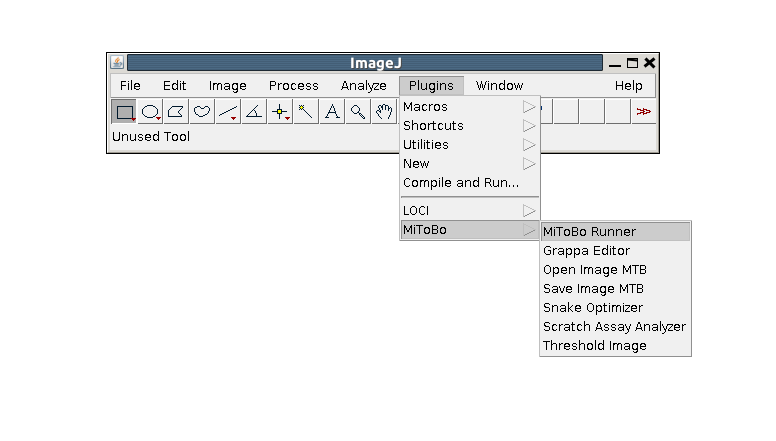
\includegraphics[width=0.85\textwidth,clip,trim= 0 0 0 30]{../images/ScreenshotImageJ_trans.png}
\vspace*{-1.7cm}
\caption{\label{fig:imageJ}Screenshot of ImageJ's plugin menu including \mitobo's submenu.}
\end{center}
\vspace*{-0.25cm}
\end{figure}
\end{center}

\vspace*{-0.75cm}
As mentioned above the key component for accessing \mitobo's functionality from within ImageJ is
its operator runner. Fig.~\ref{fig:oprunner} shows a screenshot of its main window after it has 
been invoked from ImageJ's plugin menu\footnote{\mitobo also offers a toolbar button and an associated start-up macro
to enable direct access to the operator runner, please refer to the installation instructions on the webpage for details on 
how to setup the button.}.

\begin{wrapfigure}[19]{r}{0.5\textwidth}
\vspace*{-1.6cm}
\begin{center}
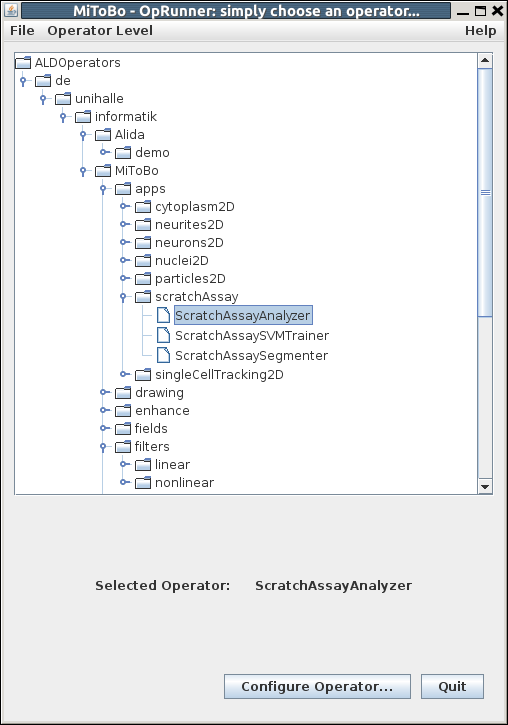
\includegraphics[width=0.475\textwidth]{../images/ScreenshotOpRunner.png}
\vspace*{-0.45cm}
\caption{\label{fig:oprunner}Screenshot of \mitobo's operator runner.}
\end{center}
\end{wrapfigure}
The operator runner basically displays a hierarchical menu of all available \alida and \mitobo
operators, organized according to their Java packages. From this menu you can select the 
operator of your choice, either by simply double-clicking on its name, or by selecting the entry
and clicking the 'Configure Operator \ldots' button at the bottom of the window. 
Subsequently \mitobo will launch a control window 
for the selected operator which allows you to configure and execute the operator you have chosen. 
Note that in \mitobo two different categories of operators are available. On the one hand there
are operators optimized for use by non-experts and often of general interest, while on the 
other hand it also subsumes a large collection of more sophisticated and often quite specific
operators. You can switch the operator selection menu between these categories via the 
item 'Operator Level' in the menubar on top of the window.
  
%\begin{wrapfigure}[15]{r}{0.65\textwidth}
%\vspace*{-0.5cm}
%\begin{center}
%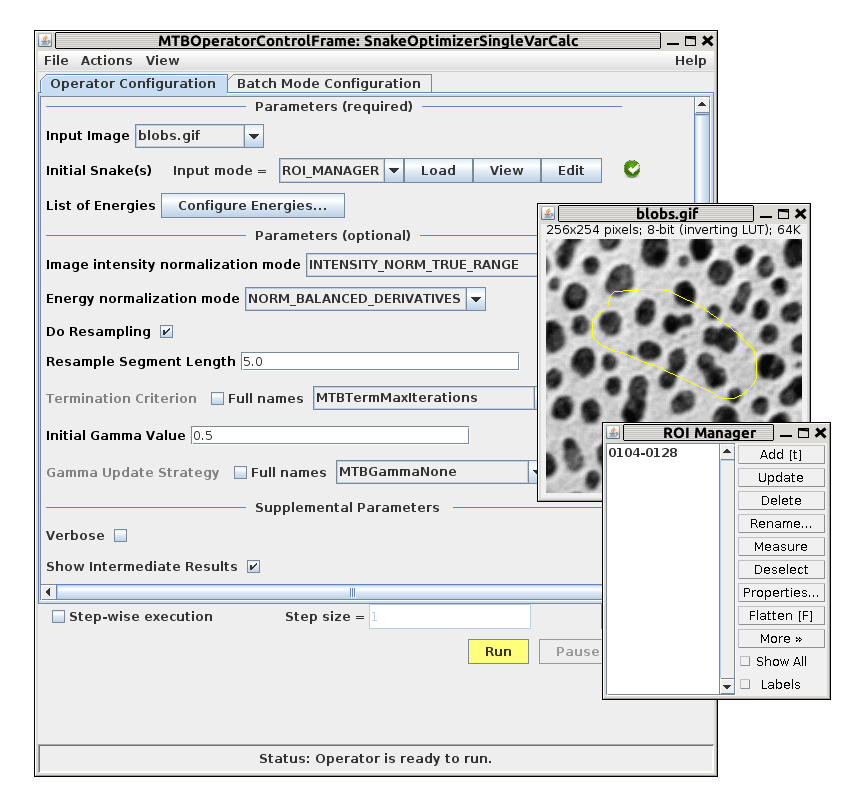
\includegraphics[width=0.6\textwidth]{../images/ScreenshotSnakeOp_trans.png}
%\caption{\label{fig:snakeop}Screenshot of the control window for the Snake Optimizer operator.}
%\end{center}
%\end{wrapfigure}
\begin{center}
\begin{figure}[t]
\begin{center}
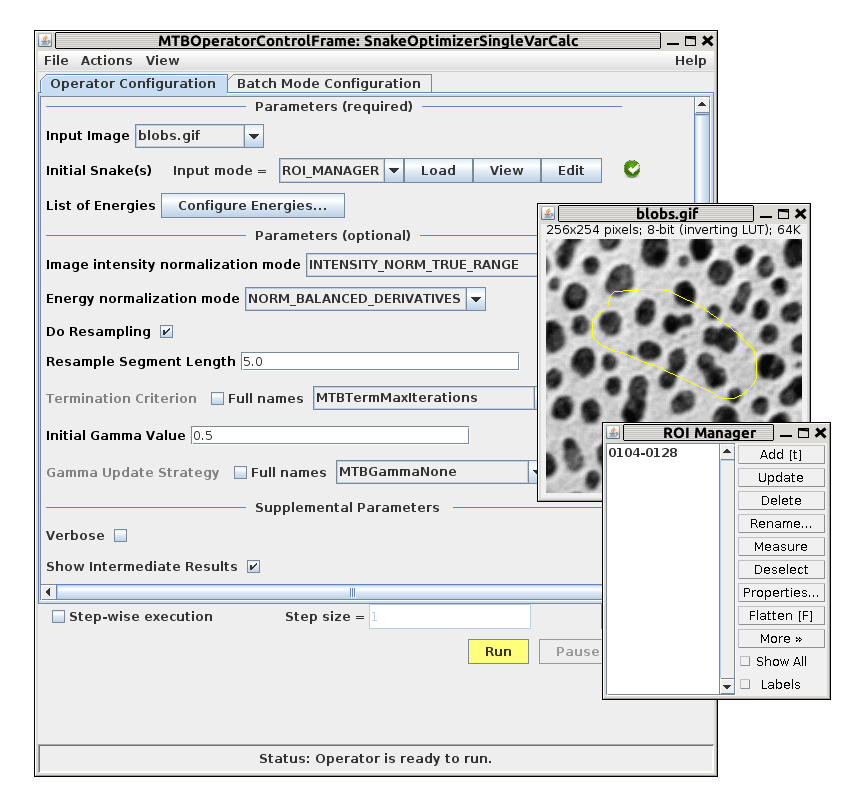
\includegraphics[width=0.85\textwidth]{../images/ScreenshotSnakeOp_trans.png}
\caption{\label{fig:snakeop}Screenshot of the control window for the 'Snake Optimizer' operator.}
\end{center}
\end{figure}
\end{center}

In Fig.~\ref{fig:snakeop} as an example the control window for the 'Snake Optimizer' operator is depicted.
It is automatically generated by the framework from the operator's source code and allows for 
operator configuration and execution. The window basically displays a panel with graphical
elements to configure all the parameters of the operator. It offers a menubar where you can 
find items for loading and saving the operator configuration, change viewing options, and also have
access to an online help for the specific operator. The help provides detailed information on the 
operator's parameters and how to configure the operator properly. The bottom section of the control
window contains control elements for executing the operator. In the simplest case there is just
a 'Run' button. More sophisticated operators, like the 'Snake Optimizer', allow for advanced user interaction.
For these operators the panel includes additional buttons, e.g., for pausing and resuming the operator. 

\label{sec:opRunImageJ}

\section{Running Operators from Commandline}
When using ImageJ or ImageJ $2.0$ it is quite natural to interact with plugins and operators, respectively, via 
graphical user interfaces. Nevertheless, quite often not only some few images need to be analyzed,
but nowadays even high-throughput processing is an important issue. While ImageJ has built-in
functionality for scripting and macros, \mitobo in addition offers a handy commandline tool by 
which all of its operators (and also ImageJ $2.0$ plugins) can directly be called from console in a
generic fashion. This way they can easily be applied to large collections of image data and also be used
from within shell scripts or comparable frameworks.  

The commandline operator runner is essentially an \alida tool, i.e.~is to be found in the package
{\tt de.unihalle.informatik.Alida.tools.OpRunner}. Its basic usage is as follows:
{\small
\begin{center}
{\tt java  de.unihalle.informatik.Alida.tools.OpRunner  <operator name>  \{
parameter=value\}}
\end{center}
}
Its first argument is the name of the operator class to be executed. You do not need to specify its complete 
package name, but the simple class name by itself is usually sufficient. Moreoever, the commandline 
operator runner also supports auto-completion if the given prefix is unique among all operators 
and plugins found on the classpath.  

Following the operator name the commandline operator runner expects a set of 'name=value' pairs 
for the parameters of the operator. While the parameter names are defined by the operator's 
member variables (execute the operator runner with option '-n' to only print its parameters), 
the exact 
syntax of the value strings depends on the data types of the parameter and their data I/O providers. 
For native data types and 
strings it is sufficient to simply provide the concrete values, for image data types a filename
is required from where to load the image. The following example illustrates this by calling 
an operator for image erosion:
{\small
\begin{center}
{\tt java de.unihalle.informatik.Alida.tools.OpRunner ImgErode inImg=test.tif
masksize=3}
\end{center}
}
However, the commandline operator runner and its built-in parser also support far more complex 
calls to operators. To illustrate this, below the call to an extended snake segmentation operator
is shown. The operator {\tt 'SnakeOptimizerCoupled'} allows to apply multiple simple snake 
optimizer operators of type 
{\tt 'SnakeOptimizerSingleVarCalc'} simultaneously to one image, given by the parameter 'inImg'. 
The operator among others takes a prototypical operator object 
of type {\tt 'SnakeOptimizerSingleVarCalc'} as input parameter ('snakeOptimizer'). This object 
by itself expects, e.g., a weighted set of energies ('energySet') which is formed by a collection 
of energy objects ('energies') and an array of corresponding weights ('weights'). The energy
objects can again be parametrized, e.g., in the example below the energy object of type 
{\tt 'MTBSnakeEnergyCD\_CVRegionFit'} defines two parameters {\tt lambda\_in} and {\tt lambda\_out}:
\begin{center}
\hspace*{-1cm}{\tt java  de.unihalle.informatik.Alida.tools.OpRunner 
SnakeOptimizerCoupled $\backslash$ }\\
{\tt  initialSnakes=RoiSet.xml inImg=cell.tif outSnakes=snakesOut.xml $\backslash$}\\
\hspace*{-1.25cm}{\tt snakeOptimizer='\$SnakeOptimizerSingleVarCalc:\{energySet= $\backslash$}\\
{\tt \{energies=[\$MTBSnakeEnergyCD\_CVRegionFit:\{lambda\_in=1.0,$\backslash$}\\
\hspace*{9cm}{\tt lambda\_out=5.0\}],$\backslash$}\\
\hspace*{-7.5cm}{\tt weights=[1.0]\}\}'}
\end{center}

For accessing the results of an operator invoked by the commandline runner it is required to 
specify targets for the operator's output parameters. In case of the image erosion operator it provides
its result through an output parameter denoted 'resultImg'. Consequently, to save the eroded image to 
file it is sufficient to extend the operator call as follows: 
\begin{center}
{\tt java  de.unihalle.informatik.Alida.tools.OpRunner ImgErode inImg=test.tif
$\backslash$\\
\hspace*{5cm} masksize=3 resultImg=result.tif}
\end{center}
Note that output parameters for which no target is provided will be ignored by the commandline 
operator runner, thus, are not available upon termination.

The examples shown above only provide you with a very brief overview of the functionality of the 
commandline operator runner. To learn more about all its options and features, please refer to 
the documentation of \alida where more details can be found.  
\label{sec:opRunCmdline}

\section{Graphical Workflow Design with Grappa}
Solving sophisticated image analysis problems usually requires to apply a combination of different
algorithms to given data to extract desired results. In ImageJ this can be
accomplished by applying a sequence of plugins sequentially or in parallel to given image data and 
record a macro of the processing steps for later reuse. \mitobo extends ImageJ's support for such 
workflows formed by multiple plugins or operators, respectively, by featuring a graphical 
editor for simplified workflow design. The editor named {\tt Grappa}, which is the acronym for 
{\em {\bf \em Grap}hical {\bf \em P}rogramming Editor for {\bf \em A}lida}, can be invoked from the plugins menu.  

In Fig.~\ref{fig:grappa} a screenshot of the Grappa main window is shown. 
The window is basically separated into
the node selection menu on the left and the workbench area on the right. In the selection menu 
all \alida and \mitobo operators (and in ImageJ $2.0$ also a subset of its plugins) are 
available as processing nodes for Grappa. The nodes in the selection menu are arranged in a 
hierarchical ordering according to their package structure. 

Workflows can be designed in the workbench area on the right. It allows to instantiate different 
workflows each being linked to an individual tab of the workbench panel. Operator nodes can be
added to a workflow either by double-clicking on the operator name in the selection menu or by 
selecting an operator and afterwards clicking once on the position in the workflow tab where the 
operator node should be positioned. Nodes can easily be dragged and repositioned as well as 
resized by mouse actions. Once different nodes have been added to a workflow, edges
can be added between ports of different nodes with the mouse to define the flow of data and control. 
All edges
are directed, always connecting an output port of one node with an input port of another. Note
that on drawing edges Grappa performs type-checking, i.e.~only ports being associated with 
compatible parameter data types can be linked to each other.
\begin{center}
\begin{figure}[t]
\begin{center}
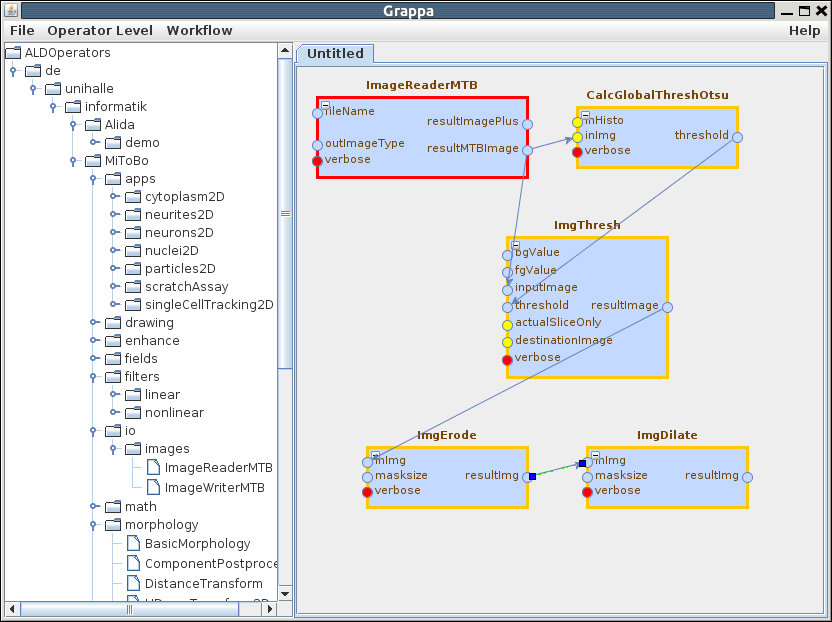
\includegraphics[width=0.85\textwidth]{../images/ScreenshotGrappa.png}
\caption{\label{fig:grappa}Screenshot of the graphical workflow editor Grappa.}
\end{center}
\end{figure}
\end{center}

\vspace*{-0.5cm}
For node configuration the mechanisms of the graphical operator runner (Sec.~\ref{sec:opRunImageJ})
are adopted. From the context menu of a node (which opens on right-clicking on the node) 
the option 'Configure\ldots' is available by which a graphical configuration window pops up.
The window is essentially identical to the control window which is displayed by the operator 
runner except that the control section is missing. All parameter values can easily be edited via
the graphical components of the window.

Nodes in a workflow can have different states indicated by the color of their border. Red framed
nodes are not ready for execution, i.e.~their configuration is not complete. If a node is readily
configured and can directly be executed its border has a yellow color, while nodes that are 
configured, however, require additional input data from preceeding operator nodes (like most of 
the nodes in Fig.~\ref{fig:grappa}) have an orange color. Prior to executing these orange nodes it
is, thus, necessary to execute the preceeding nodes first. Grappa takes care of such 
dependencies, i.e.~automatically executes nodes first from which result data is required for 
proper workflow or node execution.
After successful execution of a node its color 
changes to green indicating that result data is available. These data can graphically be examined 
via the node's context menu from which a result window can be opened. 
Note that Grappa updates the state of a node in 
real-time, i.e.~each change in its configuration or state is directly mirrored by its border color.

For executing a workflow Grappa offers different modes. Either a complete workflow can be 
executed or just a fraction of it up to a certain node. To run the complete workflow use the
corresponding item from Grappa's menubar or right-click on an empty place in the workflow tab and
select the related option from the context menu which is shown. To only partially run a workflow
select the corresponding option from the context menu of the node until which you would like to 
execute the workflow. Nodes having green color cannot be executed again until their configuration 
is changed.

Apart from the basic functionality for workflow design Grappa offers some additional convenience 
functions to simplify working with the editor. For example workflows can be saved to 
and read from disk. They can be renamed to meaningful names, and also a complete reset of a 
workflow in terms of deleting all nodes is possible. For more information on Grappa please refer
to the Alida documentation and its user and programmer guide.

\label{sec:grappa}

\section{Accessing and Exploring History Graphs}
One of the main features of \mitobo and \alida, respectively, is their capability of automatically documenting data processing
pipelines. The operator concept allows to get a detailed internal log of all data manipulations, which
can subsequently be used to convert the
process history into a directed graph data structure denoted {\em history graph} in the following.
 
The \mitobo\ operator concept defines operators as the only places where data are processed and manipulated. 
Each call to an operator is associated with a certain configuration of the operator, defined by its {\em parameters}. 
The operator receives a number of objects as input parameters, 
which for example may be images or segmentation results like regions. The behaviour of the operator is controlled by control 
parameters, for example the size of a structuring element or a threshold. 
Finally, the operator produces output data, in particular images, but also for example numerical data,
regions or contours.

In \mitobo\ an image analysis pipeline usually consists of a set of different operators that are applied to incoming data and
produce result data. The order in which the operators work on the data depends on the specific pipeline. The invocation of
operators can be of pure sequential nature or subsume parallel processing steps. In addition, a nested application
of operators is possible. Given this principle each analysis pipeline and its
data flow may be interpreted
and visualized as a directed acyclic graph (cf.~Fig.~\ref{fig:DAG} for an
example).

A \mitobo\ history graph basically consists of operator and data nodes which are connected by edges 
indicating the flow of data, as can be seen from Fig.~\ref{fig:DAG}. 
The figure shows a screenshot of \mtbc which is a graph visualization tool derived from {\em Chisio}\footnote{
Chisio website, \href{http://sourceforge.net/projects/chisio}{http://sourceforge.net/projects/chisio}}.
Chisio is a graph visualization and editing tool written in Java which we extended for the specific needs of \alida and 
\mitobo history graphs.
More detailed information about \mtbc and its installation and usage can be found on the \alida webpage and in particular 
in \alida's user guide.

Within the history graph each operator node, which is linked to the {\em call} of a specific operator,
is depicted as a rectangle with the operator's 
classname in the bottom line,
For each input and output parameter object the operator node features input and output ports which may be conceived as the entry or exit points of data into and out of the operator. These ports are depicted as filled ellipses in light green (input ports) and dark green (output ports),
respectively. Each input port has exactly one incoming edge, while an output
port may be connected to multiple target ports,
depending on where the data is passed to. In Fig.~\ref{fig:DAG} the result
image 'resultImg' produced in the {\tt MTBMedian}
operator is handed over to the {\tt ActiveContours} operator as well as
returned directly to the calling operator
{\tt CellSegmentation}. Each port of an operator has an individual name indicating the input or output object associated
with the port. This allows to distinguish between ports if one operator defines multiple input ports as is
the case for the {\tt ActiveContours} operator.
\begin{center}
\begin{figure}
\vspace*{-0.85cm}
\centerline{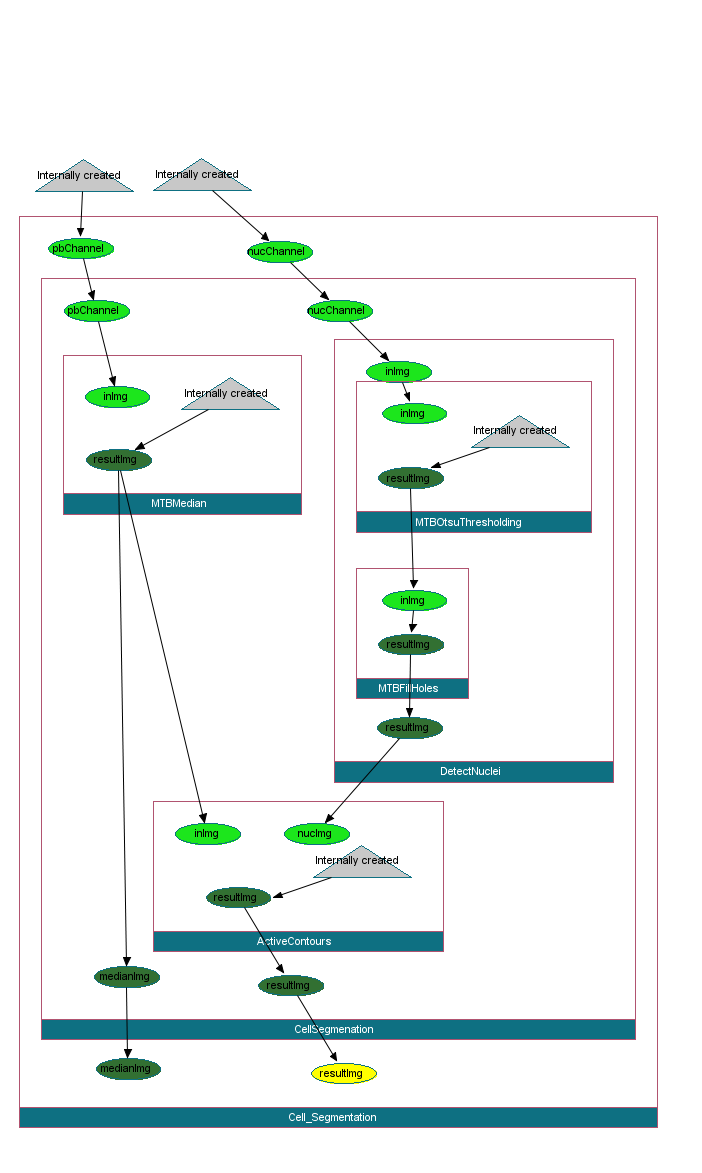
\includegraphics[clip, trim= 0 0 20 110, width=0.9\textwidth]{../images/exampleDAG.png}}
\vspace*{-0.85cm}
\caption[Example of a history graph.]{\label{fig:DAG}
A \mitobo\ history graph: the directed acyclic graph represents the application of nested operators. 
Calls to operators are depicted as rectangles, input and output ports as ellipses filled in light or dark green,
respectively. 
The grey triangles relate to newly generated data objects, and the yellow ellipse indicates the result data object
to which this history graph is linked to.}
\end{figure}
\end{center}

\vspace*{-1.25cm}
In addition to operator nodes and their ports there are also data nodes in the graph 
corresponding to the creation of new data objects, e.g., when data is read from
file, cloned or generated from scratch. These are depicted as triangles filled
in light grey.
In Fig.~\ref{fig:DAG} two data objects are created outside of the
processing pipeline as a result of reading images (at the top of the figure) and
are passed as input data objects to the {\tt Cell\_Segmentation} operator. 
Additionally, three more images are created by the operators {\tt MTBMedian}, {\tt MTBOtsuThresholding} and {\tt
ActiveContours} which in all three cases form the resulting data objects of these operators
and are passed to the outside via output ports.

Fig.~\ref{fig:DAG} shows the history graph for the output object 'resultImg' of
the operator {\tt Cell\_Segmentation}, where the corresponding port is shown as
a yellow ellipse at the bottom of the figure.
This history subsumes the calls of seven operators in total where some of these
calls are nested. The outmost operator is {\tt Cell\_Segmentation} which was
implemented as a \mitobo\ plugin, indicated by the underscore in its name
(cf.~Chap.~\ref{chap:ImplPlugins}). This plugin calls the {\tt CellSegmentation}
operator implementing the actual algorithms. For cell segmentation two input
images are required whereas one of these images is median
filtered by {\tt MTBMedian} while the second one is fed into the {\tt
DetectNuclei} operator. Inside of that operator
first {\tt MTBOtsuThresholding} is called, and the binary result image is subsequently post-processed applying {\tt
MTBFillHoles}. Its result is handed back to the calling {\tt DetectNuclei} operator and also directly propagated further back
to the {\tt CellSegmentation} operator. This operator finally calls the {\tt ActiveContours} operator which
generates one of the two result images of {\tt CellSegmentation}. The second result image is the median
filtered image which is also returned to the calling plugin as mentioned above.

The history data is stored in XML format in a file accompanying the actual data object file. 
The format basically relies on {\em GraphML}\footnote{GraphML website, 
\href{http://graphml.graphdrawing.org/}{http://graphml.graphdrawing.org/}} with some \alida and \mitobo\
specific extensions. When reading and writing images using \mitobo's {\tt 'Open\_Image\_MTB'} and {\tt 'Save\_Image\_MTB'} plugins,
or directly its {\tt 'ImageReaderMTB'} and {\tt 'ImageWriterMTB'} operators, respectively, history files are automatically considered. For example, for an image stored in the file '{\tt
example.tiff}' its history data is automatically saved to the accompanying file
'{\tt example.ald}'. The extension '{\tt
.ald}' indicates a {\em \mitobo\ processing history} file and in fact is derived from \alida, which is responsible for the 
processing histories in \mitobo. When later on reading the image using {\tt 'Open\_Image\_MTB'} or {\tt 'ImageReaderMTB'},
\mitobo's open operator checks for an accompanying file, and if one is found it is read and the corresponding history data is linked to the
image object. This allows to trace the processing history of an object in the
long run and even when the
processing pipeline was interrupted by intermediate savings of data to disk.

Note, the identity of images is {\em not} preserved in the processing history
across file boundaries. If two (or more) input images for the current top
level operator (in Fig.~\ref{fig:DAG} this would be the operator {\tt Cell\_Segmentation}), are loaded
from the same image file, both will nevertheless be displayed as different data
nodes in the history. The reason is that object identity is not -- and maybe even cannot -- be checked from the
processing history of former operations.

\paragraph{Important Note:}
At the moment, with regard to ImageJ, automatic process documentation is only supported for operators and plugins from
\mitobo\ itself, i.e.~intermediate calls to pure ImageJ functions are not documented and may corrupt the processing history. 
Contrary, in ImageJ $2.0$ also calls to ImageJ $2.0$ plugins are included in the history. But note that in both cases,
to make use of the automatic documentation to its full extent, it is indispensable to use the I/O operators of \mitobo\ to open 
input data and save the resulting output data as the ImageJ and ImageJ $2.0$ I/O functions do not know anything about histories. 

\label{sec:history}

